\chapter{Introduction} \label{ch:introduction}

A Genetic Algorithm (GA) is a biologically inspired form of computing.  GAs can be used for many different purposes, from optimization to classification to design and testing.  They can be applied anywhere that a solution can be encoded and then autonomously evaluated.  However, they are most well understood as a general solution to optimization as a form of stochastic gradient descent, similar conceptually to simulated annealing. In this paper, I attempt to narrow the role of GAs as they pertain to pattern recognition and classification.  In the remainder of this chapter I will describe GAs in general terms and discuss the motivations of this paper.  In chapter 2, I will discuss the specifics of the GAs which I use in this paper in detail.  In chapter 3 I will describe the experiments conducted and discuss the results.  In Chapter 4 I will describe future avenues of study which are available. 

\paragraph{Genetic Algorithms Introduction}
Imagine a colony of rabbits.  The rabbits are quite content to munch on clovers and thistles and the like.  Some rabbits are much more content than others, and have significant girth.  One day foxes find the rabbits. There are many more rabbits than foxes, and the foxes can't eat all of them.  The heaviest rabbits are both the slowest and the most appetizing to the foxes, and they are the first to go, but many die.  They have failed the evolutionary filtering process.  However, the rabbits that survive are thinner, and the most successful are likely faster.  These are the rabbits which survive to populate the next generation.
\\GAs encapsulate this process, though usually with much less mayhem.  The algorithm is as follows:
\begin{lstlisting}[language = algorithm, caption={Basic GA}, label={fig:basicga}]
Population := RandomInitialization()
	while True:
		for each Solution in Population:
			Evaluate Solution
			Assign Fitness to Solution
		newPopulation = SurviveAndBreed(Population)
		Population = newPopulation
	end while
\end{lstlisting}

\subparagraph{Stopping Conditions} This algorithm can run for a predetermined number of generations, indefinitely, or until another specific criterion is met.  Consider the problem of finding a way of combining 4 operands with 3 operators to achieve a particular value.  There are often many ways to solve this problem.  If one was to use a GA to solve the equation, the algorithm could stop as soon as it had valid solution values for a, b, c, d, and the 3 operators which satisfied the equation.  For example:
\begin{align*}
		a \: op_1\: b\: op_2\: c\: op_3\: d &= x\\
		3 \times 7 \times 3 + 5 &= 68\\
		9 \times 7 + 8-3 &= 68
\end{align*}
\subparagraph{Solution Encodings}
Now lets look specifically at what is meant by a solution.  First, GAs usually have some encoding based ultimately on a string of 0s and 1s, called a bitstring\footnote{Other genetic alphabets are possible as well, though less common.}. Continuing with our example, we know that there are 4 operands which have a value between 0 and 9, or 10 values total.  To encode that in a bitstring we use the values 0000-1010.  We could also include some error correcting code to randomly reassign the bits if they go outside of the values, ensuring that any solution randomly generated contains valid data (we could also use more bits and/or arbitrarily assign values via modulo arithmetic, but this is the most instructive method for our current purposes).  Next, we have the operators, which can be $+$, $-$, $*$, or $/$.  These fit nicely within the 00-11 bit range, with no need of error correction.  So we have a bitstring with the form xxxx-xx-xxxx-xx-xxxx-xx-xxxx\footnote{We use the hyphens here only for readability.  The bitstrings contain only 1s and 0s.}, 22 bits which satisfy the constraints of our problem. The second line of the above example would be 0011-10-0111-10-0011-00-0101.
\subparagraph{Fitness Functions}
Following along with the algorithm,\begin{flushleft}
	
\end{flushleft} we need to assign fitness.  In this case the closer one is to the solution, the better, usually \footnote{There are examples of x where this won't work as well; in a shortened version of our example problem, for instance, if the target is 25, $2\times3\times4$ will quickly dominate the fitness landscape but isn't actually any closer to a valid solution than $5\times5+9$.}.  There is research showing that a fitness function should be differentiable, at least as far as the solution space.  Point discontinuities aren't an issue if they occur outside of the solution space, which is important for us because we're going to make use of one. Specifically, the function 
\begin{equation*}
F(s) = \frac{1}{|E(s)-x|}
\end{equation*}
Where E(s) is the result returned by evaluating s, the numeric string.  So if we had the string 3-6*6+2, then E(s)= -16.  Assuming x is still 68, then the fitness for that particular s would be \(\frac{68}{84}= 1.19E-2\), extremely low. When 
E(s) = x or F(s) = ${\infty}$
we break out of the infinite loop.  This would be a discontinuity, but the function is still differentiable across where we're evaluating it.
\subparagraph{Breeding and Survival}
Now that we have a fitness function, we can evaluate the entire population and determine who has the highest fitness.  With a random seed, the first generation is usually not very fit.  Regardless, the next step is to see who survives and who breeds into the next generation.
Survival is usually an arbitrary matter of copying the best solution(s) \textit{in toto} to the next generation.  \footnote{Some variations have ages, where all solutions will live a certain amount of time, and more fit solutions have longer lifespans than less fit solutions.  These will not be covered further in this document.}  This is typically referred to as elitism, and it is usually a percentage around 10\% of the population that is uncritically copied into the next generation.  Properly done, this guarantees monotonically non-decreasing fitness of the best solution from one generation to the next.\\
The next step is to pick some fraction of the population as breeding stock.  The most fit are generally given preferential treatment, but not exclusive preference.  This is in large part because in GAs as in life, genetic diversity is a critical trait to the overall fitness of a population.  For GAs, it means that diversity speeds convergence to ensure that even the less fit have a chance to propagate into the next generations.  The method we employ, a fairly standard one, is Roulette Uniform Selection.  To get an intuition for the algorithm, see ~\ref{fig:rusillustration}.  In it, you can see that RUS chooses markers (represented by the arrows) equally spaced between the beginning of the population and the end.  Everywhere a marker falls means a copy of that solution gets passed into the breeding population for the next generation.  This is usually guaranteed to get at least 1 copy of the most fit individual, but everything else is based on chance.  \\
There is some discussion that suggests that proportional selection provides the weakest selective pressure of several types of selection processes and thus that other methods should be employed or that supplementary approaches be taken\citep{back_selective_1994}. While we have found this to be true to some extent selective pressure that is too strong can cause premature convergence\citep{affenzeller_self-adaptive_2003}, we implemented tournament selection, linear selection, and a Biased Random Key selection scheme \citep{ruiz_biased_2015} before settling on RUS because in testing the GA would typically converge to minima prematurely.  Thus we are actively choosing to preserve diversity over rapid but premature convergence.
\begin{figure}
	\centering
	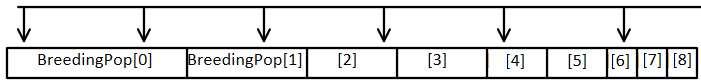
\includegraphics[width=0.7\linewidth]{figures/png/RUSIllustration}
	\caption[Roullete Uniform Selection]{An example of RUS. The bar represents the cumulative fitness of the population. The arrows represent which members of the population go on to become a breeding member.  In this example, 3 gets skipped even though it has higher fitness than 4 and 6, while 0 gets copied into the breeding population twice.}
	\label{fig:rusillustration}
	
\end{figure}
\\
With a breeding population in place, we can begin the breeding process.  This is typically accomplished via an operation called crossover, which I will explain below.  \\
\begin{tabular}{|c|c|c|c|c|c|c|c|}
	\hline
	\textit{A} & \textit{1001} & \textit{10} & \textit{0011} & \textit{11} & \textit{1001} & \textit{00} & \textit{0111}\\ 
	\textbf{B} & \textbf{0011} & \textbf{01} & \textbf{1000} & \textbf{01} & \textbf{0001} & \textbf{10} & \textbf{1001}\\
	\hline
\end{tabular}\\
We begin with two solutions.  Crossover takes and returns 2 bitstrings.    It also has several subtypes, which I will illustrate in sequence.  First is one-point crossover.  This means that before crossing, a crossover point is chosen and offspring are produced as a copy, and when this point is reached, the offspring cross over and begin taking material from the other parent.  \\

\begin{tabular}{|c|c|c|c|c|c|c|c|}
	\hline
	\textit{A'} & \textit{1001} & \textit{1}\textbf{1} & \textbf{1000} & \textbf{01} & \textbf{0001} & \textbf{10} & \textbf{1001}\\ 
	\textbf{B'} & \textbf{0011} & \textbf{0}\textit{0} & \textit{0011} & \textit{11} & \textit{1001} & \textit{00} & \textit{0111}\\
	\hline
\end{tabular}\\

Two point crossover is similar to one point, except that crossing happens twice.\\

\begin{tabular}{|c|c|c|c|c|c|c|c|}
	\hline
	\textit{A'} & \textit{1001} & \textit{10} & \textit{00}\textbf{00}  & \textbf{01} & \textbf{0001} & \textbf{10} & \textbf{1}\textit{111}\\ 
	\textbf{B'} & \textbf{0011} & \textbf{01} & \textbf{10}\textit{11} & \textit{11} & \textit{1001} & \textit{00} & \textit{0}\textbf{001}\\
	\hline
\end{tabular}\\

Notice that here the final digit of A' and the second digit of B' become invalid (1111 is not between 0000 and 1001). This case is not controlled for in Crossover, but rather handled later by evaluating the offspring in the catch-all error function which is invoked before evaluation.

The final standard type is uniform crossover, which makes a check at each bit to crossover.  It results in much more mixing, depending on the probability of a crossover event.  One advantage is that it treats the beginning and end as the same, which can't be said for either of the first two.  Another is that it allows the designer to specify, directly and exactly, how much gene mixing should occur on average.

One thing that might be noticed is that regardless of where the crossover point is, with these methods if both A and B contain a particular bit in the same location, it will appear in both offspring.  This is one reason that diversity is important:  if the population becomes too homogeneous, it will be unable to change except through random mutation, which we discuss shortly.\\
One other form of crossover we will deal with is one that counters this potential vulnerability.  It is a shifted crossover, so that one bitstring shifts forward a random number of bits, and then crossover proceeds normally.
\\
Other forms of crossover are possible, though they are not as widely represented in the literature.  One is a modified uniform crossover that checks to cross only  at each ``word", that is at each column representing a digit or operator in our example.  This gives the designer some control over how much contiguous information is exchanged per crossover.  Other variations with three or more parents, or even random asexual reproduction are possible.  Logical operations are viable, though again care must be taken to not increase homogeneity overmuch. \\

\subparagraph{Mutation}
Mutation is fairly straightforward.  Usually after crossover and before insertion in the next generation, that is, only affecting the offspring of breeding and not elitism, each bit in the bitstring has a chance to change.  The algorithm is perhaps the most instructive: \begin{lstlisting}[language=algorithm, caption={Mutation}, label={fig:mutation}]
for (Solution s in Crossover(A,B)):
	for each bit in s.Bits:
		if(MutationChance > Random(0,1)) bit = !bit
	end for
end for
\end{lstlisting}
There are some implementations that vary in that they will change random values to 1 or 0 rather than flipping bits (in other words, values will change about half as often).  A standard value for mutation is small, about 
${\frac{1.0}{Solution.Length}}$ which means on average 1 bit will change per solution per generation.\\
What is less straightforward are the effects of mutation over a population.  While values of 0 often stagnate in local minima, an upper correlate doesn't seem to exist.  That is, one could set mutation high, say 25\%, and turn off crossover entirely, and proceed with elitism and mutation alone and arrive at solutions.  In practice, this is much slower than using crossover. A general rule of thumb is to keep mutation low, and increase it even more slowly to combat stagnation.\\
\paragraph{Drawbacks}
While GAs have great versatility, there are some drawbacks which significantly limit their utility.
\subparagraph{Swiss-Army Chainsaw}
First, GAs are not the perfect solution for anything.  At their core, they are a biased-walk\footnote{With a random-walk on one side of the spectrum and a guided approach, such as gradient descent, on the other.}.  This means that while they will come to a local optima, there is no guarantee they will achieve a global optimum.  If there exists a tailored solution for a problem, using that will probably work faster and better.
\subparagraph{And Quick to Anger}
Second, GAs are subtle things.  The fitness function, not given its due in this writeup, can be the difference between a quickly converging solution and processors spinning their wheels for days or months coming to one sub-satisfactory solution after another.  A GA will optimize the fitness function, and that's all it will do.  So if you want to maximize a metric, say accuracy for a classifier, be aware that it might do exactly that by simply guessing the most prevalent answer in the dataset.  This will get it to a local optima, and it might be surprisingly difficult to get it out of it.\\
Furthermore, there are hyperparameters which effect the GA directly but can be difficult to tease out.  What should the elitism percent be?  It probably depends on your other parameters.  There are ways of optimizing these, and they themselves might be amenable to a further GA, except that evaluating them is time consuming; should your fitness function be speed of convergence?  Or the best solution arrived at within 100 generations?  That might seem too long, but use fewer generations and you run the risk of invoking too much sensitivity to starting conditions to draw meaningful conclusions.  There are some rules of thumb to assist with these situations, but they only mitigate the problem, they don't eliminate it entirely.
\subparagraph{Toolset}
Finally, a GA is only as good as its toolbox.  On Earth, that toolkit was physics.  All of physics, and massively, embarrassingly parallel at that.  That's difficult to take advantage of digitally, where you not only have the responsibility of developing an encoding but also defining the universe your population lives in.  For instance, the heart of this paper is whether to use a GA to optimize a classifier or to use a GA to classify things.  The classifier has theory underpinning its toolkit, the GA has only whatever fitness function and encoding it is supplied.  Or, to get back to our example, it might speed convergence to increase mutation rates and restrict crossover to occur only at the breakpoints of binary words.  The downside of this is that GAs are supposed to be able to solve any problem, and while they can, they also require a certain amount of customization to not waste everyone's time.  The harder the problem, the more customization that is usually required.  And at that point, if a tailored solution of some kind exists it's probably easier to code up and implement than an equivalent GA.  At their core, the GA is a biased walk, but building in paths will hopefully make that walk much quicker.
\paragraph{Theoretic Underpinnings}
Intuition is often insufficient for or even anathema to scientific inquiry, and so far that is all we have relied upon to understand why GAs work.  The Fundamental Theorem of Genetic Algorithms is used to explain much of it.  First, where we explicitly represent populations as collections of bitstrings, we may impose an additional ordering on them, the schema.  Returning to our example, consider the equations: \begin{align*}
3 \times 7 \times 3 + 5 &= 68\\
9 \times 7 + 8 - 3 &= 68\\
9 \times 7 + 6 \times 2 &= 75
\end{align*}  
These translate to the bitstrings
\begin{align*}
0\textbf{0}1\textbf{1-10-0111-}&1\textbf{0}-0011-00-\textbf{0}101\\
1\textbf{0}0\textbf{1-10-0111-}&0\textbf{0}-1000-01-\textbf{0}011\\
1\textbf{0}0\textbf{1-10-0111-}&0\textbf{0}-0110-10-\textbf{0}010
\end{align*}
Let's just assume that our x is close to, but is not 68.  Let's say it's 71.  This means that each of these bitstrings will have a relatively high fitness.  Specifically, the first two have a fitness of $\frac{1}{|71-68|}=\overline{.3}$ and the third has a fitness of .25.   However, a close inspection of all bitstrings side-by-side shows that they have a considerable amount of overlap.  All begin with odd numbers multiplied by seven, etc.  You can see the overlapping sections in bold, but pay careful attention to the long contiguous sequence.
Schemata are a way of considering a population theoretically.  A schema introduces a third character into the alphabet of bitstrings:  an * indicating either 1 or 0.  Schemata are of any length, and may be defined by their offset and bitstring (their length may be obtained from their bitstring).  Thus, offset 0 and ``***1-10-0111-**" is a valid schema which describes both solutions.  In fact, there is one schema that describes both strings, which is already represented by retaining the symbols where it is bold and replacing it with * where they don't match.\\It should be obvious that doing any calculations with schemata are infeasible, simply because for even short bitstrings, the possible schemata to describe the population increase exponentially. Let m be the length of a bitstring, and S be the set of schemata which can describe the population.  Then let \begin{equation*}
	|S|=\sum_{i=1}^{m}3^i(m-i+1) = \frac{3}{4}(-2m+3^{m+1}-3)
	\end{equation*}
While we could try to constrain this by only using the schemata that describe the currently existing population, that problem is also exponential, and potentially worse computationally, because any member of the population has $$\sum_{i=1}^{m}3(m-i+1) =\frac{3}{2}m(m+1)$$ schemata that describe it, but then these would need to be compared with the sets generated by all $2^n$ combinations of members of the population.\\
However, feasibility of computation aside, we can use this to gain a further and more formal understanding of how GAs function.\\
Informally, if we assume that schemata describe our population, whatever they may be specifically, we may also assume that short, more fit schemata will have a greater than average fitness than is represented in the population, and as such these short, fit schemata are likely to increase in representation throughout the population.  Shorter schemata will survive because longer schemata are more likely to be broken up by crossover. 
Three more concepts need to be understood before the equation itself: First,  is the order of a schema H, which is the number of non-wildcard bits it contains.  Higher is more specific.  Second is the defining length, which is the distance between the first and last non-wildcard bits.  If we return to our example, and let $\schemaSymbol_a$= offset 0, ``***1-10-0111" and $\schemaSymbol_b$= offset 0, ``*0*1-10-**11", then $\schemaOrder{\schemaSymbol_a} = \schemaDefiningLength{\schemaSymbol_a}=7$, while $\schemaOrder{\schemaSymbol_b} = 6$ and $\schemaDefiningLength{\schemaSymbol_b} = 8$.  Third is $\schemaFitness{\schemaSymbol}$, which describes the average fitness of a schema.  This is defined as 
$$\schemaFitness{\schemaSymbol}=\sum_{s\epsilon \schemaAsFunction{P}}^{}\frac{\fitnessFunction{s}}{|\schemaAsFunction{P}|}$$ where H(P) is the schema H applied to the population P, which returns a subpopulation of solutions, and where s is one such solution returned.
   \\With these concepts understood, the Fundamental Theorem of Genetic Algorithms is as follows: \begin{align}
\schemaRepresentation{H}{t+1}&\geq \schemaRepresentation{H}{t} \frac{\schemaFitness{\schemaSymbol}}{\averageFitness}\bigg[1-\bigg(\crossoverRate+\schemaOrder{H}\mutationRate\bigg)\bigg]
\end{align}
Where $\averageFitness$ is the average fitness of the population at time t.  $\crossoverRate$ and $\mutationRate$ are probabilities of crossover and mutation, respectively, and $\schemaRepresentation{H}{t}$ is the number of representations of a schemata H at a time step t in a population.  The type of crossover plays a role, here.  Depending on implementation, in single point crossover the probability of crossover occurring is usually 1\footnote{Often, at any rate.  When it isn't, it can be used as a sort of ersatz elitism, simply passing copies of both parents into the next generation.  However, if employing a significant level of elitism, there's a good chance at least one parent is already in the population, and doing this would create a duplicate, which is a waste of a slot in the population.}
.  Instead, a random number from 1 to L is usually chosen, with each index being equally likely, and crossover occurs at that index. Thus, for single point crossover, $$\crossoverRate^{SinglePoint} = \frac{\schemaDefiningLength{H}}{L-1} $$ For two point crossover, the odds of breaking a given schema is much more likely, because it is the outcome of 2 events not happening, that is $$\crossoverRate^{TwoPoint} = 1-\frac{L-\schemaDefiningLength{H}}{L-1} \frac{L-\schemaDefiningLength{H}}{L-2} $$ from which we get the general $$\crossoverRate^{NPoint} = 1- \frac{(L-\schemaDefiningLength{H})^n}{\frac{(L-1)!}{(L-1-n)!}} $$
for n point crossover. \\Uniform crossover is implemented differently, and is generally done with a rate, which we'll call $\gamma$.  Since this is the case, it makes calculating $\crossoverRate$ more straightforward.  
$$\crossoverRate^{Uniform} = 1 - \gamma^{\schemaOrder{H}} $$So, while representations for schema which are more fit than others will increase over time, the particular type of crossover can have a significant impact on how much representation they gain.  It is worth noting that a uniform crossover with even a moderate rate of crossover (say, .3) can rapidly lead to the eradication of all higher-order schemata.  Also worth noting is that when a schema applies to both solutions, both offspring will also belong to that schema using standard crossover methods.  Finally, if an implementation includes a probability other than 1 for any of the forms of n point crossover, that probability is simply multiplied to the appropriate $\crossoverRate$.\\
A few observations about this function.  As overall length of the bitstring increases, the inhibition of single-point crossover decreases, but inhibition of n point crossover generally increase, and if the mutation rate is linked inversely to length then it does as well.  Uniform crossover is less directly linked to length, though not independent: as L increases, the numbers of higher order schemata increase exponentially.  Survival of a particular schema becomes very unlikely without a strong selective pressure toward retention. Further, high order and fitness schemata with greater defining lengths rapidly become unlikely to obtain except through elitism.  
\\
\paragraph{Motivations}
Over the course of researching how GAs were being used in recent times a broad pattern emerged.  With regards to classification, there were two basic schools of thought:  one in which GAs were used to optimize classifiers and one which used GAs as classifiers directly.  Both camps have \textit{prima facie} impressive examples of these approaches.  Thus, this project was born: to attempt to answer which approach is more generally applicable.\\
GA are widely used for numerous purposes, but we seek to ascertain their suitability for pattern recognition, specifically classification.  In this paper, we attempt to determine how suitable GAs are for the task of classification.  To determine credibility, we propose 3 tests.  First, we will run a GA on the datasets acting directly as a classifier.  Second, we will run two classifiers, a lone Decision Tree, and a Naive Bayes classifier with default settings as a control.  Finally, we will run the same classifiers optimized through a GA which will run for a modest number of generations.  We will collect confusion matrices from the resulting classifiers and compare them.\\
To ensure that our approach is generally applicable, we propose datasets from divergent fields of study and with data in different configurations.  With minimal adjustments, the program we have written is capable of automating this process over almost any dataset, but we have chosen 3 from the UCI repository\citep{lichman_uci_2013} : Yeast Dataset (Yeast)\citep{paul_horton_uci_1996}, Bach's Chorales Dataset (Bach)\citep{daniele_p._radicioni_uci_2014}, and Cardiotocography Dataset (Cardio)\citep{j._p._marques_de_sa_uci_2010}.  This gives us 4 different configurations to use, as Cardio has two modes that it runs in, with the pattern class code (1-10) or the fetal class code (Normal, Suspect, Pathologic), which we refer to as Cardio and CardioNSP, respectively.  This gives us data from biology, music, and medicine, which serves as a broad start.  However, we are also making the code available in in its entirety for anyone who wants to extend this to other domains of study.\\
\subparagraph{Priors}
Going into this project, a case for either side could be made.  On the case for the Pure GA approach you have a few points.  First and foremost, versatility:  the GA is only limited by the encoding, and a clever encoding could exploit nuances that people wouldn't be likely to notice in the data.  Secondly, there's something about the simplicity of only having 1 component to debug: this could speed development which would mean more effort could be spent developing the encoding and the fitness function.  One con is the inverse of the first pro, that encoding needs to exploit the nature of the data, and so much time can be spent customizing the approach to the data, but this is also antithetical to the idea of a generic solution to classification, so whatever encoding we use must be good enough to apply to many problems.\\
For the Hybrid camp, the pros are primarily that the GA gets to leverage the theoretical robustness of the external classifier.  That is to say that there has been a great deal of work to make classifiers extremely good at what they do and writing a GA to compete with or exceed beyond that work is difficult.  There are several cons, though; the external classifier needs to be written and debugged separately and then in conjunction.  Also, there are now 2 or more entities to be maintained which means much less time can be spent on any one project, unless you simply tie into some other classification package, though that may have its own challenges.\\
Thus, before going into this project, we slightly favored the hybrid approach.  But we wanted to make sure that there was plenty of versatility for the GA to make use of, so for the implementation of our pure GA we settled on CellNet \citep{kharma_project_2004}, which is a variable length GA which has a new breeding operator.  We discuss this project in depth in Chapter 2.  

\paragraph{Literature Review}
\subparagraph{Hybrid Approach}In \cite{schuman_spatiotemporal_2014} they use classifiers to breed numerous neural networks in parallel and test them against MNIST.  In \cite{ocak_medical_2013} the authors use a support vector machine (SVM) optimized by a GA to predict fetal well-being, with considerable success.  In \cite{marchetti_improving_2013} GAs were used for feature selection and then the features generated were passed to a logistic regression classifier.   In \cite{wu_evolving_2015} GAs were used in conjunction with particle swarms to optimize a neural network for predicting rainfall.  While GAs performed better in conjunction with the particle swarms than alone, the idea of using a GA to build a better classifier is present.  \cite{chou_optimizing_2014} and \cite{duan_characterization_2014} discuss using a GA to optimize another SVM, this time emphasizing the mileage obtained from leveraging the SVM for curve fitting while the GA handles the optimization of the SVM itself.  \cite{devos_simultaneous_2014} takes a similar approach, but instead focuses on using the GA to determine which combination of preprocessing methods to use.  The GA is also used to determine two meta parameters for the SVM itself.  Once these are determined, the SVM is used to handle the classification.  In \cite{uysal_text_2014} they use GAs to focus their Latent Semantic Indexing approach on promising semantic features.  They use two different approaches and find that both are much more effective on a wide range of tests than the approach without the GA optimization. \cite{salari_novel_2014} used an ensemble approach which is quite novel.  First, they use doctors to decide which features of the datasets in question to use.  Then, they give these features to a Feed Forward Neural Net(FFNN) on one hand and a GA on the other.  The GA generates several different arrays of features, and then these arrays and the results from the FFNN are fed to a k nearest neighbor to find fuzzy classes, then those classes are iteratively pared down until they are no longer fuzzy.  They apply their model to multiple datasets, and compare across a wide variety of methods with a variety of metrics, over which they show statistically significant gains on nearly every method, metric, and dataset.  \cite{alexandre_hybridizing_2015} hybridizes a GA with an Extreme Learning Machine, with considerable gains in both binary and multiple class classification over several learning methods.


\subparagraph{Purist}
Here, we look at papers where GAs act directly as the classifier.  We have included papers where rules for classification are generated.  \cite{dehuri_application_2008} uses two different GA approaches to classification rule generation, one a simple one similar to the  ``canonical" approach and one a multi-objective optimizer.  The multi-objective GA performed well, though areas for improvement were discussed in the conclusion.  One area particularly limiting the GA was the number of attributes the GA was working with.  The interestingness of the discovered rules was quite high, though sometimes the comprehensibility was lacking.  Still, the rules were highly predictive on the datasets employed.
In \cite{kozeny_genetic_2015} they used 3 GAs to calculate credit scores, and compared their accuracies.  While they achieved interesting results with their methods, the most promising one scales at $O(2^L)$, which makes it unfeasible for computation except on short feature sets.  In \cite{srikanth_variable-length_1995} variable length GAs are used to draw fuzzy ellipses in a decision space, and thresholding is used to make the borders crisp.  This approach is shown to be comparable over their selected dataset to a back-propagation neural net (BPNN).\\
\cite{fidelis_discovering_2000} uses a GA to develop rules for diagnosing breast cancer and dermatology.  They achieve 95\% accuracy on the dermatology but only 67\% on the breast cancer, which is, by the author's own admission, a much more difficult dataset with a great deal more noise.  Beside the results, the rules themselves were of interest, and evolved 3 separate times from different random seeds.   The rules developed seemed to hit the knowledge discovery trifecta of predictiveness, comprehensibility, and interestingness.\\
In \cite{hoque_implementation_2012} and \cite{li_application_2012}, GAs are used to solve an intrusion detection problem.  While both papers boasts a discovery rate of nearly 100\%, if one ignores the denial of service attacks their discovery plummets.  Unfortunately, it isn't clear that the authors are entirely at fault for this; the data which might have been used\footnote{The authors don't elaborate and there are several versions of the KDDCup data.} for the DARPA challenge contained 5,283 non-DoS attacks, but 391,000 DoS attacks (it also contained 97,000 non-attacks).  It’s small wonder that the GAs would optimize according to capture the most numerous classes in the data.
\cite{tseng_genetic_2008} is another example of rule discovery, but this time applied to land-cover classification.  They specifically use a GA as an alternative to other methods such as a Neural Net(NN) or other Bayesian classifiers because the GA has shown that the rules it discovers are more comprehensible, even if less predictive.  In other words, while NNs may be good at solving a problem, exactly how they solve it is not always clear, and that can be problematic for many domains.  Unfortunately, while they get good accuracy they don't do a head-to-head comparison.  One possible reason is because the database is very small, at only about 400 samples.\\
Finally, we will discuss the CellNet family of papers which inspired one prong of our approach in much more detail in Chapter 2.  In the original CellNET paper \citep{kharma_project_2004} , they used a variable length GA to classify the \cite{cedar_cedar_2002} database.  While they obtained modest results, the stated goal of CellNet was to develop a GA which could approach any dataset with minimal intervention.  They continued in \cite{kowaliw_cellnet_2004}, where they employed two populations of competitive solutions called hunters and prey, where hunters are trying to classify a handwritten digit from the CEDAR database and prey are trying to obscure said image.  The results in this paper were much more impressive, and their overfitting problem diminished significantly as well.